\subsection{Work Breakdown Structure}
In this subsection you will find the main packages of our revised work breakdown structure.

\subsubsection{Pre-Study}
This package contains sub-packages for most the basic work done in the preliminary studies phase, before the start of implementation. The total number of hours in this package is 174, or about 9 person days per person.
\begin{longtable}{|p{0.7cm}|p{3cm}|p{1.8cm}|p{2.5cm}|p{2cm}|p{2.8cm}|}
\hline
\# & Sub-package & \# persons & Hours/person & Total \# of hours & Person-days (ca 5h)/persons assigned\\ 
\hline
1.1 & Choice and study of software/tools & 4 & 2 & 8 & 0.4\\ 
\hline
1.2 & Technology learning and acclimatization & 4 & 25 & 100 & 5\\ 
\hline
1.3 & Overall planning/management & 4 & 8 & 32 & 1.6\\ 
\hline
1.4 & Role distribution & 4 & 1 & 4 & 0.2\\ 
\hline
1.5 & Process/Sprint planning & 4 & 5 & 20 & 1\\ 
\hline
1.6 & Standards & 1 & 2 & 2 & 0.4\\ 
\hline
1.7 & Milestone planning and review & 4 & 2 & 8 & 0.4\\ 
\hline
\caption{WBS: Pre-Study}
\end{longtable}

\newpage
\subsubsection{Requirements}
This package consists of the gathering and analysis of functional and non-functional requirements. The total number of hours in this package is 10, or 1 person day per person.
\begin{longtable}{|p{0.7cm}|p{3cm}|p{1.8cm}|p{2.5cm}|p{2cm}|p{2.8cm}|}
\hline
\# & Sub-package & \# persons & Hours/person & Total \# of hours & Person-days(ca 5h)/persons assigned\\ 
\hline
2.1 & Functional requirements & 4 & 2.5 & 10 & 0.5\\ 
\hline
2.2 & Non-functional requirements & 4 & 2.5 & 10 & 0.5\\ 
\hline

\caption{WBS: Requirements}
\end{longtable}

\subsubsection{General Project Management}
This package contains sub-packages related to project and group management, such as meetings and managing plans. The total number of hours in this package is 152, or 7.6 person days per person.
\begin{longtable}{|p{0.7cm}|p{3cm}|p{1.8cm}|p{2.5cm}|p{2cm}|p{2.8cm}|}
\hline
\# & Sub-package & \# persons & Hours/person & Total \# of hours & Person-days(ca 5h)/persons assigned\\ 
\hline
3.1 & Meetings with customer(s)  & 4 & 3 & 12 & 0.6\\ 
\hline
3.2 & Advisor meetings  & 4 & 5 & 20 & 1\\ 
\hline
3.3 & Meeting with the group (internal meetings not directed towards other packages) & 4 & 5 & 20 & 1\\ 
\hline
3.4 & Underway administration & 4 & 20 & 80 & 4\\ 
\hline
3.5 & Plan maintenance/updating & 4 & 5 & 20 & 1\\ 
\hline

\caption{WBS: General Project Management}
\end{longtable}

\subsubsection{Architecture}
This package contains sub-packages for the design and documentation of the software architecture. The total number of hours in this package is 55, or 5 person days per person.
\begin{longtable}{|p{0.7cm}|p{3cm}|p{1.8cm}|p{2.5cm}|p{2cm}|p{2.8cm}|}
\hline
\# & Sub-package & \# persons & Hours/person & Total \# of hours & Person-days(ca 5h)/persons assigned\\ 
\hline
4.1 & Overall architecture & 2 & 10 & 20 & 2\\ 
\hline
4.2 & Detailed architecture & 3 & 5 & 15 & 1\\ 
\hline
4.3 & Patterns & 2 & 5 & 10 & 1\\ 
\hline
4.4 & Quality Attributes & 2 & 5 & 10 & 1\\ 
\hline
\caption{WBS: Architecture}
\end{longtable}

\subsubsection{Technical/API documentation}
This package contains the sub-packages related to the creation and review of the technical documentation. The total number of hours in this package is 33, or 3.4 person days per assigned person.
\begin{longtable}{|p{0.7cm}|p{3cm}|p{1.8cm}|p{2.5cm}|p{2cm}|p{2.8cm}|}
\hline
\# & Sub-package & \# persons & Hours/person & Total \# of hours & Person-days(ca 5h)/persons assigned\\ 
\hline
5.1 & Standards & 1 & 5 & 5 & 1\\ 
\hline
5.2 & Writing & 2 & 10 & 20 & 2\\ 
\hline
5.3 & Review & 4 & 2 & 8 & 0.4\\ 
\hline
\caption{WBS: Technical Documentation}
\end{longtable}

\newpage
\subsubsection{Documentation - Weekly report}
This package contains all sub-packages related to the creation of the weekly reports for the meetings with our advisor. The total number of hours in this package is 16, or 0.8 person days per person.
\begin{longtable}{|p{0.7cm}|p{3cm}|p{1.8cm}|p{2.5cm}|p{2cm}|p{2.8cm}|}
\hline
\# & Sub-package & \# persons & Hours/person & Total \# of hours & Person-days(ca 5h)/persons assigned\\ 
\hline
6.1.1 & Agenda & 4 & 1 & 4 & 0.2\\ 
\hline
6.1.2 & Hours planned \& work done & 4 & 2 & 8 & 0.4\\ 
\hline
6.1.3 & Finalization & 4 & 1 & 4 & 0.2\\ 
\hline
\caption{WBS: Weekly Report}
\end{longtable}

\subsubsection{Final Report}
This package consists of the writing of the various parts of this final report. The total number of hours in this package is 210, or about 11.5 person days per person.
\begin{longtable}{|p{0.7cm}|p{3cm}|p{1.8cm}|p{2.5cm}|p{2cm}|p{2.8cm}|}
\hline
\# & Sub-package & \# persons & Hours/person & Total \# of hours & Person-days(ca 5h)/persons assigned\\ 
\hline
7.1 & Pre-study & 4 & 12.5 & 50 & 2.5\\ 
\hline
7.2 & Architecture & 2 & 10 & 20 & 2\\ 
\hline
7.3 & Documentation & 4 & 20 & 80 & 4\\ 
\hline
7.4 & Implementation & 4 & 15 & 60 & 3\\ 
\hline
\caption{WBS: Final Report}
\end{longtable}

\newpage
\subsubsection{Implementation - Webassistenten}
The sub-packages in this package are the parts of implementation related to the interoperability of our product with the customer's already existing system \\ \emph{Webassistenten}. The total number of hours in the package is 30, or 3 person days per assigned person.
\begin{longtable}{|p{0.7cm}|p{3cm}|p{1.8cm}|p{2.5cm}|p{2cm}|p{2.8cm}|}
\hline
\# & Sub-package & \# persons & Hours/person & Total \# of hours & Person-days(ca 5h)/persons assigned\\ 
\hline
8.1 & Enable display of available products (no GUI is to be implemented) & 2 & 5 & 10 & 1\\ 
\hline
8.2 & Listing the next 5 available booking dates for a selected product & 2 & 5 & 10 & 1\\ 
\hline
8.3 & Listing modules available for a selected product & 2 & 5 & 10 & 1\\ 
\hline
\caption{WBS: Implementation - Webassistenten}
\end{longtable}

\newpage
\subsubsection{Implementation - Import-System Service}
This package contains the sub-packages that are the parts of implementation related to importing files and data, and placing the data into the database. The total number of hours in the package is 60, or 6 person days per assigned person.
\begin{longtable}{|p{0.7cm}|p{3cm}|p{1.8cm}|p{2.5cm}|p{2cm}|p{2.8cm}|}
\hline
\# & Sub-package & \# persons & Hours/person & Total \# of hours & Person-days(ca 5h)/persons assigned\\ 
\hline
9.1 & Receiving pdf-file and save in correct folder & 2 & 5 & 10 & 1\\ 
\hline
9.2 & Putting accompanying data in Webassistenten database (table “prospekt”) & 2 & 10 & 20 & 2\\ 
\hline
9.3 & Checking accompanying data for required fields & 2 & 5 & 10 & 1\\ 
\hline
9.4 & Placing an order in the internal order system & 2 & 10 & 20 & 2\\ 
\hline\caption{WBS: Implementation - Import-System Service}
\end{longtable}

\newpage
\subsubsection{Implementation - Miscellaneous}
This package contains the rest of the sub-packages related to implementation. The total number of hours in the package is 200, or 17 person days per assigned person.
\begin{longtable}{|p{0.7cm}|p{3cm}|p{1.8cm}|p{2.5cm}|p{2cm}|p{2.8cm}|}
\hline
\# & Sub-package & \# persons & Hours/person & Total \# of hours & Person-days(ca 5h)/persons assigned\\ 
\hline
10.1 & Database communication interface (Entity Framework) & 2 & 10 & 20 & 2\\ 
\hline
10.2 & Bugfixing & 2 & 30 & 60 & 6\\ 
\hline
10.3 & Workarounds & 2 & 30 & 60 & 6\\ 
\hline
10.4 & Testing & 4 & 15 & 60 & 3\\ 
\hline
10.5 & Underway learning & 4 & 20 & 80 & 4\\ 
\hline
\caption{WBS: Implementation - Miscellaneous}
\end{longtable}

\newpage
\subsubsection{Setup and Maintenance of Development Tools and Resources}
Because of the sheer number of various development tools and versions of those tools we had to install and use, we created a package for the installation and maintenance of these tools. The total number of hours in this package is 88, or 4.4 person days per person.
\begin{longtable}{|p{0.7cm}|p{3cm}|p{1.8cm}|p{2.5cm}|p{2cm}|p{2.8cm}|}
\hline
\# & Sub-package & \# persons & Hours/person & Total \# of hours & Person-days(ca 5h)/persons assigned\\ 
\hline
11.1 & Database Setup & 4 & 10 & 40 & 2\\ 
\hline
11.2 & Visual Studio Setup and Installation & 4 & 5 & 20 & 1\\
\hline
11.3 & Version control system & 4 & 2 & 8 & 0.4\\ 
\hline
11.4 & Configuration and maintenance of software packages etc. & 4 & 5 & 20 & 1\\ 
\hline
\caption{WBS: Setup and Maintenance of Tools}
\end{longtable}

\subsubsection{Totals}
The total time in in all our packages are listed in the following table.
\begin{longtable}{|p{2cm}|p{3cm}|p{3cm}|p{4.5cm}|}
\hline
\# persons & Hours per person & Total \# of hours & Person days per person\\ 
\hline
4 & 279.5 & 1118 & 55.9\\ 
\hline
\caption{WBS: Totals}
\end{longtable}

\subsection{Gantt}
\begin{table}[H]
\centering
\begin{tabular}{|c|p{8cm}|c|}
\hline
\textbf{\#} & \textbf{WBS Package} & \textbf{Size (Whole days)}\\ 
\hline
1 & Pre-study & 9\\ 
\hline
2 & Requirements & 1\\ 
\hline
3 & General project management & 8\\ 
\hline
4 & Architecture & 5\\ 
\hline
5 & Technical/API documentation & 4\\ 
\hline
6 & Documentation & 1\\ 
\hline
7 & Report & 12\\ 
\hline
8 & Implementation - Webassistenten & 3\\ 
\hline
9 & Implementation - import-system service & 6\\ 
\hline
10 & Implementation - Misc. & 18\\ 
\hline
11 & Setup and Maintenance of Development Tools and Resources & 4\\ 
\hline
 &  & \\ 
\hline
\textbf{Total:} &  & \textbf{71}\\ 
\hline\end{tabular}
\label{table:WBSdays}
\caption{\small{Size of WBS Packages in Whole Days}} 
\end{table}

\hspace{-5cm}
\begin{table}[H]
\centering
\begin{tabular}{|p{6cm}|c|c|c|}
\hline
\textbf{Gantt package name} & \textbf{Size (Whole days)} & \textbf{Start} & \textbf{Finish}\\ 
\hline
Pre-study (Includes requirements) & 9 & 21.08 & 30.08\\ 
\hline
Requirements & 1 & 30.08 & 6.09\\ 
\hline
General project management and documentation & 9 & 21.08 & 21.11\\ 
\hline
Sub-package: Overall architecture and Quality Attributes & 2 & 9.09 & 13.09\\ 
\hline
Technical/API documentation & 4 & 28.1 & 7.11\\ 
\hline
Report & 12 & 30.08 & 20.11\\ 
\hline
Sprint 1 (8, 9, 10, 4.2 and 4.3) & 10 & 16.09 & 27.09\\ 
\hline
Sprint 2 (8, 9, 10, 4.2 and 4.3) & 10 & 30.09 & 11.1\\ 
\hline
Sprint 3 (8, 9, 10, 4.2 and 4.3) & 10 & 14.1 & 25.1\\ 
\hline
Sprint 4 (8, 9, 10, 4.2 and 4.3) & 10 & 28.1 & 8.11\\ 
\hline
Setup and Maintenance of Development Tools and Resources & 4 & 21.08 & \\ 
\hline
\end{tabular}
\label{GanttPackages}
\caption{\small{Gantt Packages and Time Frames}} 
\end{table}

\begin{figure}[H]
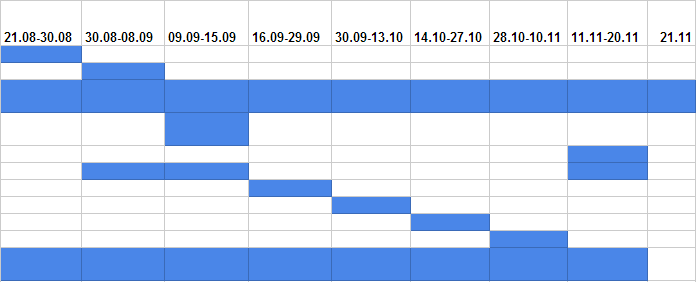
\includegraphics[width=1\textwidth]{images/gantt02.png}
\caption{Gantt Chart}
\end{figure}
